\section{Coulomb correction to the thermodynamic parameters of dense plasmas}

{\bf Coulomb interactions} we account within the Madelung approximation. The extra term in the free energy which accounts for the
electrostatic energy of each of the ions in the charge state $i$ coupled with i electrons, the latter being uniformly
distributed over the "iono-sphere"
(see Eq.(3.50) in \cite{drake}):
\begin{equation}\label{fterm}
F_M=-\frac{9}{10} \frac{q_e^2}{r_{iono}} \sum_{i=0}^{i_{max}} i^2 N_i,\qquad
r_{iono} = \left( \frac{4 \pi}{3} n_a \right)^{-\frac13}.
\end{equation}
Accordingly, in the requirement of the ionization equilibrium, $\partial F/\partial N_i - \partial F/\partial N_{i+1} - \partial F/\partial N_e = 0$ (with respect to the reaction $(i)\leftrightarrow(i+1)+e$),
the term $\partial F_{M}/\partial N_i -\partial F_{M}/\partial N_{i+1}$ will 
give the contribution of $\frac{9}{10} \frac{(2i+1)q_e^2}{r_{iono}}$ into the left hand side:
\begin{equation}
-T \log \left[ \frac{g_i}    {N_i}     e^{\sum_{j=0}^{i-1} I_j/T} \right] - \frac{9}{10} \frac{i^2     q_e^2}{r_{iono}}
+T \log \left[ \frac{g_{i+1}}{N_{i+1}} e^{\sum_{j=0}^i     I_j/T} \right] + \frac{9}{10} \frac{(i+1)^2 q_e^2}{r_{iono}}
-\mu_e = 0.
\end{equation}
The solution of the ionization equilibrium, hence, reads:
\begin{equation}
\frac{N_{i+1}}{g_{i+1}} = \frac{N_i}{g_i} \exp\left(-\frac1T \left(I_i - \frac{9}{10} \frac{(2i+1) q_e^2}{r_{iono}} + \mu_e \right)\right),
\end{equation}
or, applying this recursively and reducing the sum $\sum_{j=0}^{i-1} (2j+1) = i^2$,
\begin{equation}\label{pfM}
\frac{N_i}{g_i}=\frac{N_0}{g_0}(g_e)^i \exp \left( \frac{9}{10} \frac{i^2 q_e^2}{T r_{iono}} -\frac{\sum_{j=0}^{i-1}I_j}T \right) .
\end{equation}
This may be interpreted as the ionization potential lowering which results from the Coulomb interaction:
each of the potentials, $I_i$, is reduced by $\frac{9}{10} \frac{(2i+1)q_e^2}{r_{iono}}$.
Energy of the ion of the charge state $i$ is $E_i^* = \sum_{j=0}^{i-1}I_j - \frac{9}{10} \frac{i^2 q_e^2}{r_{iono}}$.
This effect shifts the ionization equilibrium towards higher ionization degrees, for a given temperature and atomic density.

The common multiplier, $\frac{N_0}{g_0}$, in each of Eqs.(\ref{pfM}) may be also represented as $\frac{N_a}{S}$.
From the normalization condition, $\sum N_i = N_a$, we find that $S$ is a statistical sum:
\begin{equation}
S=\sum_{i=0}^{i_{max}} g_i (g_e)^i \exp\left(-\frac{E_i^*}T\right),
\end{equation}
so that:
\begin{equation}\label{ni}
p_i = \frac{N_i}{N_a} = \frac{1}S g_i (g_e)^i \exp \left( -\frac{E_i^*}T \right).
\end{equation}

The full Helmholtz free energy now includes the contribution of the electrostatic field energy as in Eq.(\ref{fterm}):
\begin{equation}\label{fe1}
F=-T
\sum_{i=0}^{i_{max}}{
N_i\log\left[g_i
  \frac{eV}{N_i}\left(\frac{MT}{2\pi \hbar^2}\right)^{3/2}\exp \left(-\sum_{j=0}^{i-1}\frac{I_j}T \right)\right]}+F_e
  -\frac{9}{10} \sum_{i=0}^{i_{max}} N_i \frac{i^2 q_e^2}{r_{iono}}.
\end{equation}  

With the ion partition functions as in Eq.(\ref{ni}) one can rewrite Eq.(\ref{fe1}) in the following form:
\begin{equation}\label{ffullm}
F = -TN_a\log\left[\frac{eV}{N_a}\left(\frac{MT}{2\pi \hbar^2}\right)^{3/2}\right]-TN_a\log S + \Omega_e, 
\end{equation}
where, again, $\Omega_e = F_e - \mu_e N_a \sum i p_i = F_e - \mu_e N_a \langle i \rangle $.

{\bf Differentials along the curve of the ionization equilibrium} obey the equation as follows:
\begin{equation}
A_{g_e} \frac{dg_e}{g_e} = A_V \frac{dV}{V} + A_T \frac{dT}{T}
\end{equation}
\begin{equation}
A_{g_e} = \langle \delta^2 i \rangle + ZR^-(g_e), \qquad
A_T     = \frac32 Z - \frac{\langle \delta i \delta E^*_i \rangle}{T}, \qquad
A_V     = Z + \frac{3}{10} \frac{q_e^2}{T r_{iono}} \langle \delta(i^2) \delta i \rangle
\end{equation}
Again, we express the result in terms of covariances,
$\langle \delta a \delta b \rangle = \langle (a - \langle a \rangle) (b - \langle b \rangle) \rangle$,
and mean values which are now being calculated
using the modified partition functions.
Differentiation of mean values which is necessary for derivation of the above equation on
differentials is not a complicated problem with the following formula:
\begin{equation}
d \langle f_i \rangle = \left\langle \delta f_i \delta\left( \frac{dp_i}{p_i} \right) \right\rangle,
\end{equation}
where $f_i$ is a function of the only argument $i$, for example, $iE_i$ or $i^2+i$.

{\bf Plasma thermodynamics and Equation-Of-State.} 
While differentiating Eq.(\ref{ffullm}) with respect to $T$ and $V$, again, we see that the derivatives
by $g_e$ from the second and third terms cancel 
each other: $g_e(\partial \log S/\partial g_e)=\langle i\rangle=Z$,
that is evident from $d \log S = \langle d (\log p_i) \rangle$,
and $-g_eg_{e1}{\rm Fe}^\prime_{3/2}(g_e)=g_{e1}{\rm Fe}_{1/2}=Z$. That is why for the internal energy density, 
${\cal E}$, and for the pressure, $P$, we find:
\begin{equation}
{\cal E} = -\frac{T^2}V\left(\frac{\partial}{\partial T}\left(\frac F T\right)\right)=
{\cal E}_i+{\cal E}_e,\qquad{\cal E}_i=\frac32Tn_a,\qquad
{\cal E}_e = n_a\left[ \frac32 T Z R^+ + \langle E^*_i\rangle \right],
\end{equation}
\begin{equation}
P = -\frac{\partial F}{\partial V}=P_i+P_e,\quad
P_i = n_aT,\quad
P_e = n_aT ( 1 + ZR^+ - L \langle i^2 \rangle ),\quad
L = \frac{3}{10} \frac{q_e^2}{Tr_{iono}}.
\end{equation}
In the above equations we add the Madelung corrections into the energy of the electron gas, ${\cal E}_e$, and
into the pressure of electrons, $P_e$, because those corrections are controlled by the electron temperature.

However, while calculating the second order thermodynamic derivatives,
such as specific heat, the derivatives of $g_e$ essentially sophisticate the 
calculations. 

In such a way one can find the specific heat in isochoric process, per unit of volume:
\begin{equation}
C_{Ve}=\frac{\partial {\cal E}_e}{\partial T}=n_a\left[\frac{\langle\delta^2E^*_i\rangle}{T^2}+\frac{15}4ZR^+
-\frac{\left(\frac32Z-\frac{\langle\delta E^*_i\delta i\rangle}T\right)^2}{\langle\delta^2i\rangle+ZR^-}\right],
\end{equation}
the temperature derivative of pressure:
\begin{equation}
\frac {\partial P_e}{\partial T}=
n_a\left[
	\frac52 Z R^+ -
	(Z+L \langle \delta(i^2) \delta i \rangle)
		\frac{\frac32Z-\frac{\langle\delta E^*_i\delta i\rangle}T}{\langle\delta^2i\rangle+ZR^-} -
	L \frac{\langle \delta E^*_i \delta(i^2) \rangle}T
\right],
\end{equation}
as well as the isothermal compressibility:
\begin{equation}
V\frac{\partial P_e}{\partial V}=
n_a T \left[ -\frac{(Z + L \langle \delta(i^2) \delta i \rangle)^2}{\langle \delta^2 i \rangle + ZR^-} +
L \left( \frac43 \langle i^2 \rangle + L \langle \delta^2(i^2) \rangle \right) \right].
\end{equation}
For simplicity in the above equations the contributions due to ion translational motions are omitted, which are:
\begin{equation}
C_{Vi}=\frac32n_a, \qquad
\frac{\partial P_i}{\partial T}=n_a, \qquad
V\frac{\partial P_i}{\partial V}=-n_aT.
\end{equation}

Following is the table showing the values of $Z$ calculated for Xenon
at various electron temperatures
(given in electron-volts -- the value of $k_{B}T_{e}$, where $k_{B}$
is in eV/K) and heavy particle concentrations (given in number of
particles per $cm^{3}$). "no" columns contain the same values
calculated without Coulomb interation taken into account.

\begin{center}
\begin{tabular}{|c||c|c|c|c|c|c|c|c|c|c|c|c|}
\hline
Na[$1/cm^3$] & \multicolumn{2}{|c|}{$10^{18}$} & \multicolumn{2}{|c|}{$10^{19}$} & \multicolumn{2}{|c|}{$10^{20}$} & \multicolumn{2}{|c|}{$10^{21}$} & \multicolumn{2}{|c|}{$10^{22}$} & \multicolumn{2}{|c|}{$10^{23}$}\tabularnewline
\hline
Te[eV] & no & Mad & no & Mad & no & Mad & no & Mad & no & Mad & no & Mad\tabularnewline
\hline
\hline
   5. &     3.4 &     3.4 &     2.8 &     3.0 &     2.2 &     2.5 &     1.3 &     1.9 &     0.6 &     1.4 &     0.2 &     2.9\tabularnewline
\hline
  10. &     6.3 &     6.4 &     5.2 &     5.4 &     4.1 &     4.6 &     3.0 &     3.7 &     1.7 &     3.2 &     0.7 &     3.9\tabularnewline
\hline
  15. &     7.3 &     7.3 &     6.9 &     6.9 &     5.9 &     6.3 &     4.4 &     5.4 &     2.7 &     4.6 &     1.1 &     4.8\tabularnewline
\hline
  20. &     9.2 &     9.3 &     7.7 &     7.9 &     6.9 &     7.1 &     5.6 &     6.5 &     3.6 &     5.7 &     1.6 &     5.6\tabularnewline
\hline
  25. &    11.8 &    12.0 &     9.4 &     9.7 &     7.6 &     8.0 &     6.5 &     7.1 &     4.5 &     6.5 &     2.1 &     6.2\tabularnewline
\hline
  30. &    13.8 &    14.0 &    11.5 &    11.9 &     8.9 &     9.5 &     7.1 &     7.8 &     5.4 &     7.0 &     2.6 &     6.7\tabularnewline
\hline
  35. &    15.7 &    15.9 &    13.3 &    13.7 &    10.4 &    11.3 &     7.8 &     8.9 &     6.0 &     7.6 &     3.1 &     7.2\tabularnewline
\hline
  40. &    17.2 &    17.4 &    14.9 &    15.3 &    12.1 &    12.9 &     8.7 &    10.2 &     6.6 &     8.3 &     3.6 &     7.8\tabularnewline
\hline
  45. &    18.1 &    18.2 &    16.4 &    16.7 &    13.4 &    14.2 &     9.9 &    11.6 &     7.1 &     9.2 &     4.1 &     8.5\tabularnewline
\hline
  50. &    19.0 &    19.2 &    17.4 &    17.7 &    14.7 &    15.5 &    11.1 &    12.9 &     7.6 &    10.3 &     4.6 &     9.3\tabularnewline
\hline
  55. &    20.5 &    20.7 &    18.1 &    18.4 &    15.9 &    16.7 &    12.3 &    14.0 &     8.2 &    11.4 &     5.0 &    10.1\tabularnewline
\hline
  60. &    22.0 &    22.2 &    19.0 &    19.3 &    16.9 &    17.5 &    13.3 &    15.1 &     8.8 &    12.4 &     5.5 &    11.0\tabularnewline
\hline
  65. &    23.3 &    23.5 &    20.1 &    20.6 &    17.6 &    18.1 &    14.3 &    16.0 &     9.6 &    13.4 &     5.9 &    11.9\tabularnewline
\hline
  70. &    24.4 &    24.6 &    21.4 &    21.9 &    18.2 &    18.8 &    15.2 &    16.8 &    10.4 &    14.3 &     6.2 &    12.7\tabularnewline
\hline
  75. &    25.3 &    25.4 &    22.6 &    23.0 &    19.0 &    19.7 &    16.1 &    17.5 &    11.2 &    15.1 &     6.6 &    13.5\tabularnewline
\hline
  80. &    25.7 &    25.7 &    23.6 &    24.0 &    19.8 &    20.7 &    16.8 &    18.0 &    12.0 &    15.8 &     6.9 &    14.2\tabularnewline
\hline
  85. &    25.9 &    25.9 &    24.5 &    24.8 &    20.8 &    21.8 &    17.4 &    18.6 &    12.7 &    16.5 &     7.3 &    14.9\tabularnewline
\hline
  90. &    25.9 &    25.9 &    25.1 &    25.3 &    21.9 &    22.7 &    17.9 &    19.2 &    13.5 &    17.0 &     7.7 &    15.5\tabularnewline
\hline
  95. &    26.0 &    26.0 &    25.5 &    25.6 &    22.8 &    23.6 &    18.5 &    20.0 &    14.2 &    17.5 &     8.0 &    16.0\tabularnewline
\hline
 100. &    26.1 &    26.1 &    25.7 &    25.8 &    23.6 &    24.3 &    19.1 &    20.8 &    14.8 &    18.0 &     8.4 &    16.5\tabularnewline
\hline
 105. &    26.2 &    26.2 &    25.9 &    25.9 &    24.3 &    24.9 &    19.7 &    21.6 &    15.4 &    18.4 &     8.9 &    16.9\tabularnewline
\hline
 110. &    26.4 &    26.5 &    25.9 &    26.0 &    24.8 &    25.3 &    20.5 &    22.4 &    16.0 &    18.9 &     9.3 &    17.3\tabularnewline
\hline
 115. &    26.9 &    27.0 &    26.0 &    26.0 &    25.2 &    25.5 &    21.3 &    23.1 &    16.5 &    19.5 &     9.8 &    17.7\tabularnewline
\hline
 120. &    27.5 &    27.6 &    26.1 &    26.1 &    25.5 &    25.7 &    22.0 &    23.7 &    17.0 &    20.1 &    10.2 &    18.1\tabularnewline
\hline
 125. &    28.3 &    28.4 &    26.2 &    26.3 &    25.7 &    25.8 &    22.7 &    24.3 &    17.5 &    20.7 &    10.7 &    18.4\tabularnewline
\hline
\end{tabular}

\par\end{center}


%
\section{Appendix A: The Fermi function calculation approach}

For $g_e\ge1,\,\nu>-1$ the Fermi function may be developed into
convergent power series (see Eq.(5) from \cite{mcleod}):
\begin{equation}
{\rm Fe}_\nu(g_e)=\sum_{n=1}^\infty{\frac{(-1)^{n+1}}{n^{\nu+1}(g_e)^n}}.
\end{equation} 

The Taylor series in powers of $-\log(g_e)$ (see Eq.(6) from \cite{mcleod}): % from MacLeod
\begin{equation}
{\rm Fe}_{\nu}(g_e) = \sum_{i=0}^\infty{\frac{(1-2^{i-\nu}) \zeta(\nu+1-i)}{i!} (-\log(g_e))^i}.
\end{equation}
is only used for $g_e \in [e^{-3}; 1)$, because it converges when $|\log(g_e)| < \pi$.

For $0 < g_e < e^{-3}$ we use the following asymptotic series (see Eq.(8) from \cite{mcleod}): % from MacLeod
\begin{equation}
{\rm Fe}_{\nu}(g_e) \sim \frac{(-\log(g_e))^{\nu+1}}{\Gamma(k+2)} \left(1 + \sum_{i=1}^\infty{a_{2i} (\log(g_e))^{-2i}}\right).
\end{equation}
where
\begin{equation}
a_{2i} = \frac{(1 - 2^{1-2i})(k+1)!(2\pi)^{2i}}{(k+1-2i)!} \frac{|B_{2i}|}{(2i)!}.
\end{equation}
where $B_j$ denotes a standard Bernoulli number. The last formula can be simplified using the following expression for the Bernoulli numbers (see Eq.(9.616) from \cite{gradshtein}):
\begin{equation}
B_{2i} = \frac{(-1)^{i-1} (2i)!}{2^{2i-1} \pi^{2i}} \zeta(2i).
\end{equation}
so that
\begin{equation}
a_{2i} = \frac{2 (1 - 2^{1-2i}) (k+1)!}{(k+1-2i)!} |\zeta(2i)|.
\end{equation}

We only calculate the first three sum terms of the asymptotic series to get the best
approximation of ${\rm Fe}_\nu(g_e)$ for $g_e$ around $e^{-3}$:
\begin{equation}
{\rm Fe}_\nu(g_e) \approx \frac{(-\log(g_e))^{\nu+1}}{\Gamma(k+2)} \left(1 + \frac{a_2}{(\log(g_e))^2} + \frac{a_4}{(\log(g_e))^4}\right).
\end{equation}
An  asymptotic series does not guarantee an improvement in accuracy while increasing the number of the sum terms
involved. In our particular case the use of either more than or less than three sum
terms noticeably lowers the accuracy of ${\rm Fe}_\nu(g_e)$ for $g_e \in [e^{-5}, e^{-3}]$.

In both series $\zeta(x)$ denotes the Riemann zeta-function.
At $x > 0$ it can be calculated as a convergent series (see Eq.(9.522.2) from \cite{gradshtein}): % Gradshtein, Ryzhik: 9.522.2; Abramowitz: 23.2.19
\begin{equation}
\zeta(x) = \frac{1}{1-2^{1-x}} \sum_{n=1}^\infty{(-1)^{n+1} \frac{1}{n^x}}.
\end{equation}
At $x < 0$ we use the following reflection formula (see Eq.(7) from \cite{mcleod}): % MacLeod
\begin{equation}
\zeta(x) = 2^x \pi^{x-1} \sin(\frac{\pi x}{2}) \Gamma(1-x) \zeta(1-x).
\end{equation}

\begin{figure}[ht]
\centering
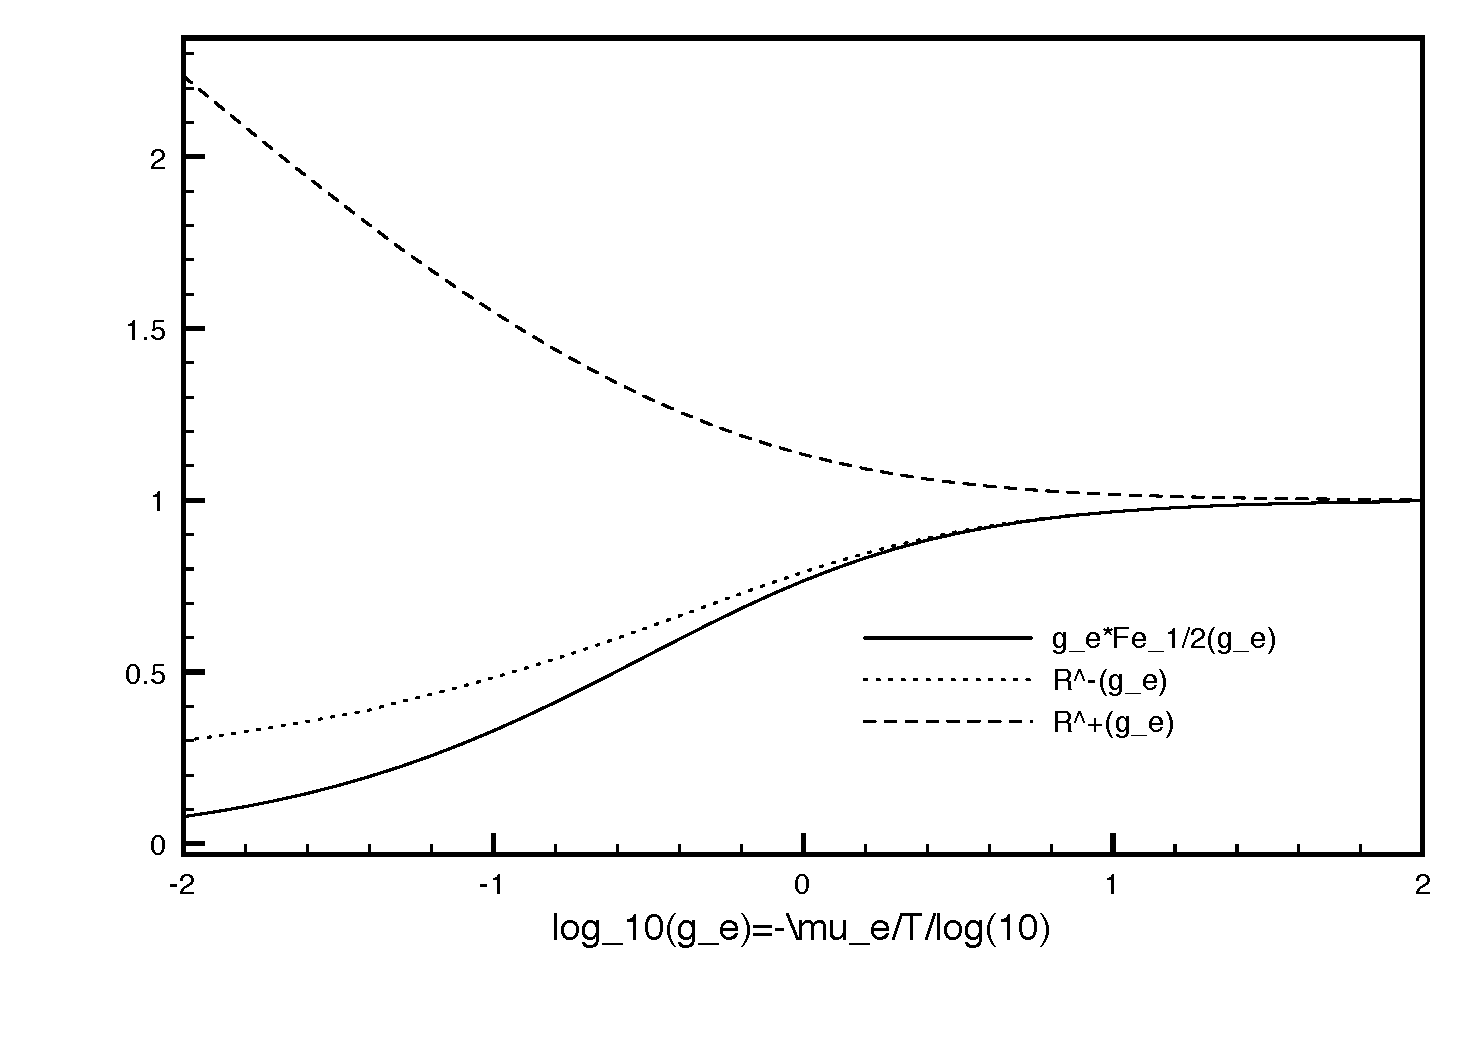
\includegraphics[scale=0.6]{FermiFunction.eps}
\caption{The Fermi function of index 1/2 multiplied by $g_e$ (solid) and the ratio functions (dashed) calculated using the described algorithm.}
\end{figure}


%\include{CoulombInteraction}


%{\bf Conclusion.} Again, mention that in the partially ionized plasma the exchamge interaction
%effect on the plasma pressure is not exhausted by the multiplier  $R^+\ge 1$, there is also the reduction in $Z$ proportional to negative 
%$\delta_{\rm Fe}$. This thermodynamical property of the partial ionized gas should be also taken into account while 
%generalizing the result for the case of small but finite Coulomb interactions, which may be  done by developing the
%chemical potential of the electron gas into a series of the average Coulomb potential of electrons.   


